
\documentclass[12pt,a4paper]{article}

\usepackage[utf8]{inputenc}
\usepackage[T1]{fontenc}
\usepackage{polski}

\usepackage{amsthm}
\usepackage{amsmath}
\usepackage{amsfonts}
\usepackage{amssymb}
%\usepackage{pgfplots}
%\usepackage{tikz}
%\usepackage{lmodern}	%fancy font
\usepackage{textcomp}

\usepackage{indentfirst}
\usepackage{graphicx}
\usepackage{caption}
\usepackage{subcaption}
%\usepackage{siunitx}
\usepackage{here}


\setlength{\textheight}{24cm}
\setlength{\textwidth}{15.92cm}
\setlength{\footskip}{10mm}
\setlength{\oddsidemargin}{0mm}
\setlength{\evensidemargin}{0mm}
\setlength{\topmargin}{0mm}
\setlength{\headsep}{5mm}
%\usepackage{tikz}
%\usepackage{lmodern}	%fancy font
\usepackage{textcomp}

\usepackage{indentfirst}
\usepackage{graphicx}
\usepackage{caption}
\usepackage{subcaption}
%\usepackage{siunitx}
\usepackage{here}
\usepackage[margin=1in]{geometry}% Just for this example
\setlength{\parindent}{0pt}% Just for this example
\setlength{\textheight}{24cm}
\setlength{\textwidth}{15.92cm}
\setlength{\footskip}{10mm}
%\setlength{\oddsidemargin}{0mm}
%\setlength{\evensidemargin}{0mm}
\setlength{\topmargin}{0mm}


\begin{document}

\begin{table}[]
\label{my-label}
\begin{tabular}{|p{7.5cm}|p{7.5cm}|}
\hline
									           					&                           \\

\includegraphics[height=3cm]{logo}             					& \textbf{Technika cyfrowa} \\ \hline
\multicolumn{1}{|l|}{\textbf{Temat ćwiczenia}} 					& \textbf{Numer ćwiczenia}  \\
\multicolumn{1}{|l|}{Minimalizacja i praktyczna realizacja złożonych funkcji logicznych}	& 2                         \\ \hline
\multicolumn{1}{|l|}{\textbf{Wykonawca}}       & \textbf{Ocena}            \\
\multicolumn{1}{|l|}{Marcin Przewięźlikokokokokokwski}          &                           \\ \hline
\end{tabular}
\end{table}

\section{Cel ćwiczenia}


Zapoznanie się z zastosowaniem tablic Karnaugh'a do minimalizacji graficznej złożonych funkcji logicznych oraz zaprojektowanie w Multisimie układu cyfrowego zwiększającego o 1 trzybitową liczbę całkowitą oraz wyświetlacza siedmiosegmentowego.

\section{Przebieg ćwiczenia}

\subsection{Układ cyfrowy inkrementujący trzybitową nieujemną liczbę całkowitą}
Dla każdego bitu wyjściowego sporządzono tablice Karnaugh'a (od bitu najstarszego do najmłodszego), gdzie bity wejściowe w kolejności starszeństwa to ABC:\\

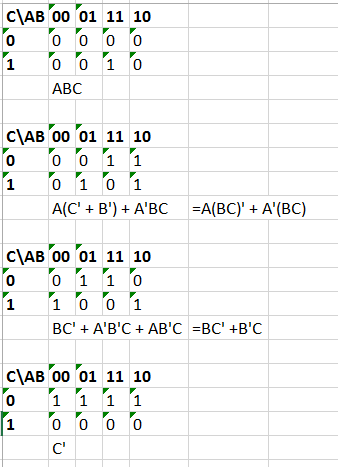
\includegraphics[scale=0.8]{2aKarnaugh}\\
Następnie w Multisimie stworzono układ odpowiadający wyprowadzeniu i przetestowano go używając wyświetlacza siedmiosegmentowego:\\
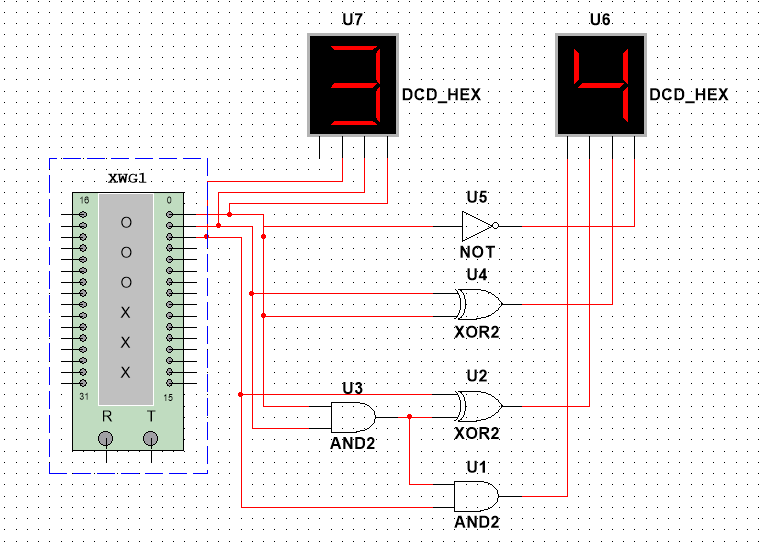
\includegraphics[scale=0.8]{2aBetter}\\

Układ można też zrealizować przy użyciu półsumatorów.


\subsection{Minimalizacja funkcji metodą tablic Karnaugha}
Zadaną funkcję logiczną przedstawiono w poniższej tabeli, a następnie zminimalizowano korzystając z metody Karnaugh'a. Wynik minimalizacji również znajduje się na poniższym zdjęciu:

\centering
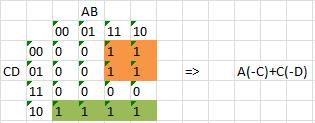
\includegraphics{2bVog}\\
\raggedright
W MultiSimie swtworzono model bramki niezminimalizowanej oraz zminimalizowanej. Porównano je Logic Analyzerem i oceniono, że minimalizacja przebiegła pomyślnie:
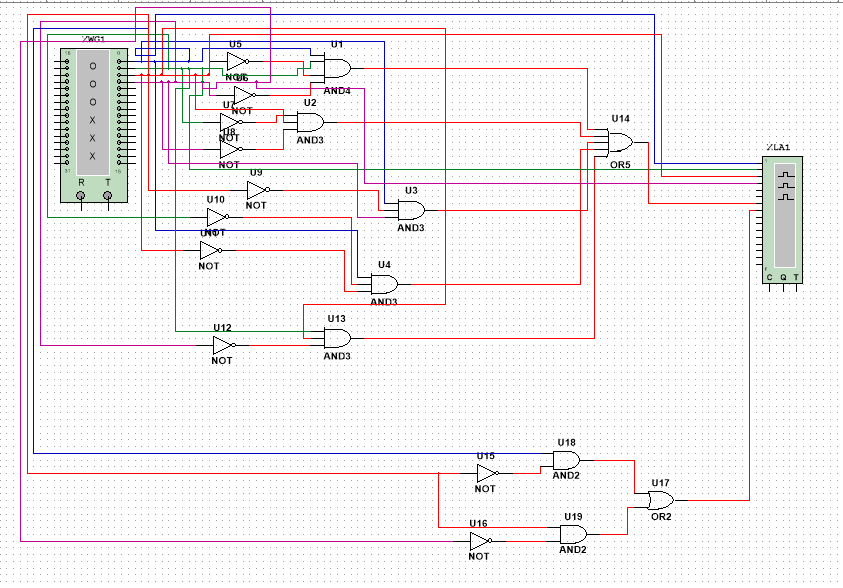
\includegraphics[width=\textwidth]{2b1}\\
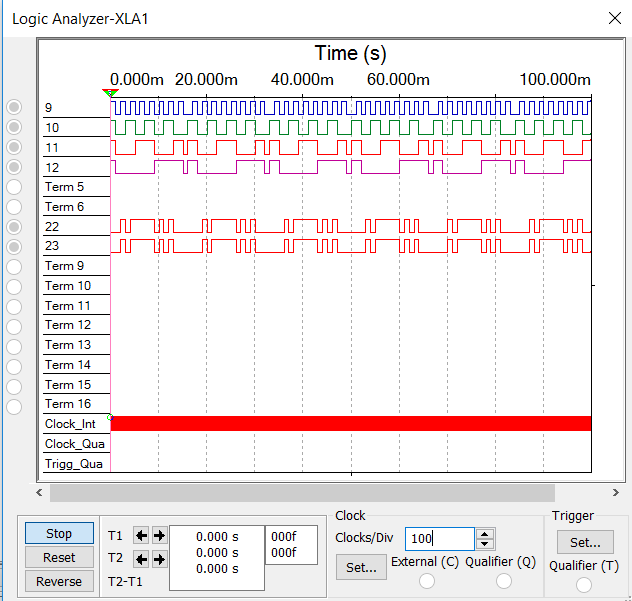
\includegraphics[width=\textwidth]{2b2}


\subsection{Transkoder czterobitowych cyfr}
\centering
W oparciu o poniższą konfigurację segmentów:


\centering
\includegraphics[scale=0.07]{7seg/segconf}

\raggedright
Dla każdego z 7 segmentów zrealizowano tablicę Karnaugh'a prezentującą pożądane zachowanie segmentu, zminimalizowano funkcję logiczną i zbudowano odpowiedni obwód:\\
\centering
\textbf{Segment a:}\\
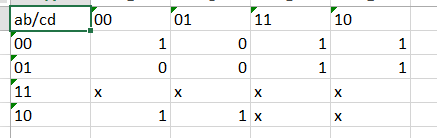
\includegraphics[scale=0.8]{7seg/seg0}\\
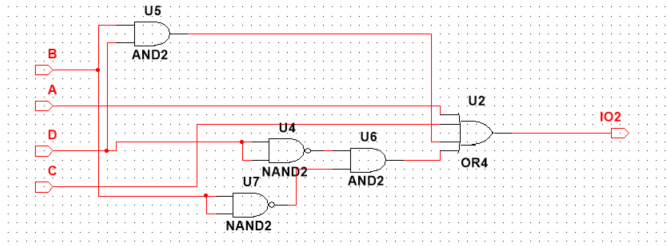
\includegraphics[scale=1]{7seg/seg0circ}\\
\textbf{Segment b:}\\
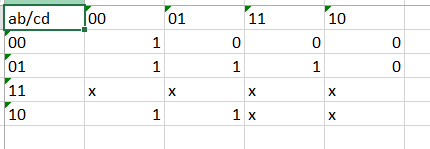
\includegraphics[scale=0.8]{7seg/seg1}\\
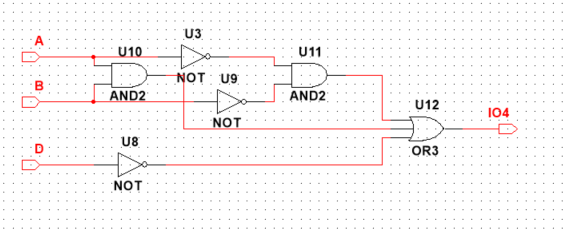
\includegraphics[scale=1]{7seg/seg1circ}\\
\textbf{Segment c:}\\
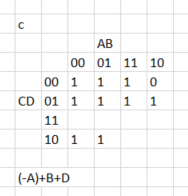
\includegraphics[scale=0.8]{7seg/seg2}\\
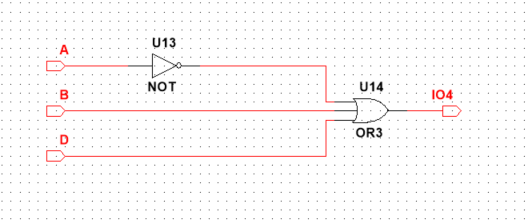
\includegraphics[scale=1]{7seg/seg2circ}\\
\textbf{Segment d:}\\
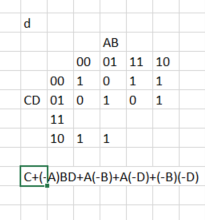
\includegraphics[scale=0.8]{7seg/seg3}\\
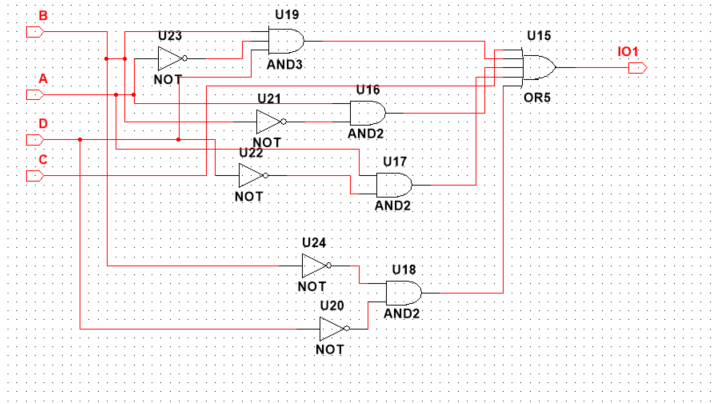
\includegraphics[scale=1]{7seg/seg3circ}\\
\textbf{Segment e:}\\
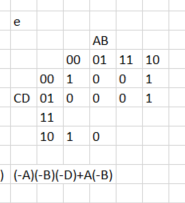
\includegraphics[scale=0.8]{7seg/seg4}\\
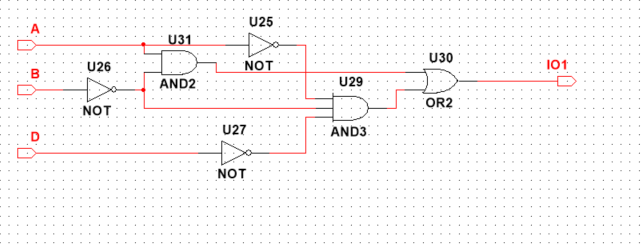
\includegraphics[scale=1]{7seg/seg4circ}\\
\textbf{Segment f:}\\
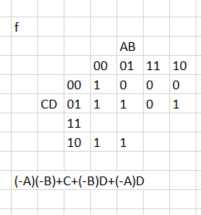
\includegraphics[scale=0.8]{7seg/seg5}\\
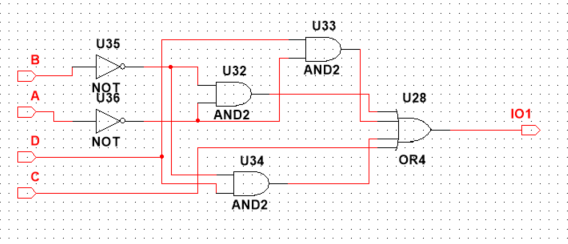
\includegraphics[scale=1]{7seg/seg5circ}\\
\textbf{Segment g:}\\
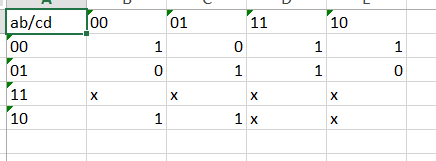
\includegraphics[scale=0.8]{7seg/seg6}\\
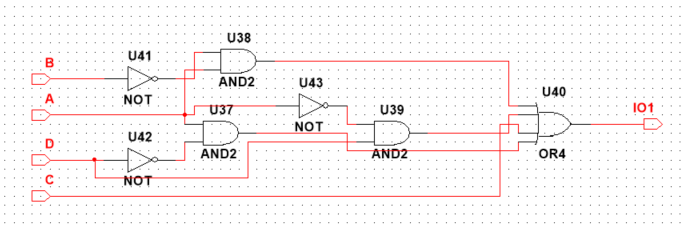
\includegraphics[scale=1]{7seg/seg6circ}\\
\raggedright

Wszystkie obwody podłączono do wyświetlacza siedmiosegmentowego i przetestowano. Wyświetlacz wskazywał przewidywane cyfry:
\centering
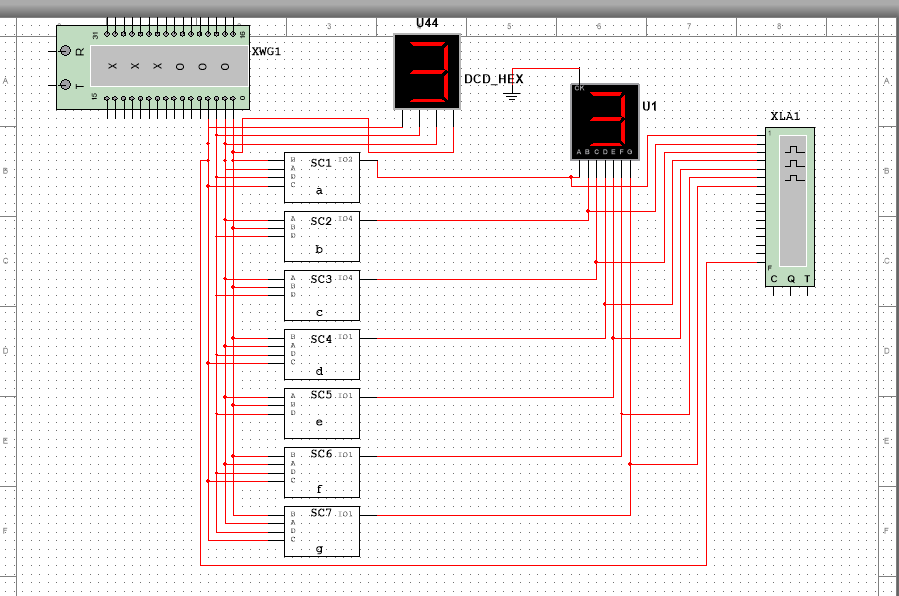
\includegraphics[width=\textwidth]{7seg/7segall}


\end{document}
